\begin{subfigure}[b]{0.24\linewidth}


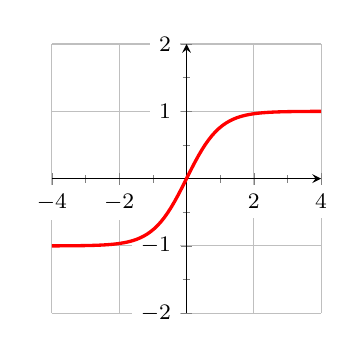
\begin{tikzpicture}
	\begin{axis}[ 
%title=$\tanh(x)$,
xmin=-4, xmax=4,ymin=-2, 
ymax=2, grid=major,
height=5cm, width=5cm,
axis line style={latex-latex},
axis lines=middle,
ticklabel style={font=\footnotesize,fill=white},
minor tick num=1,
scaled ticks=false] 
\addplot[samples=100,red,very thick] {tanh(x))};
%\addlegendentry{$\tanh(x)$}
\end{axis}
\end{tikzpicture} 
\subcaption{tanh}
\end{subfigure}
\hfill
\begin{subfigure}[b]{0.24\linewidth}



	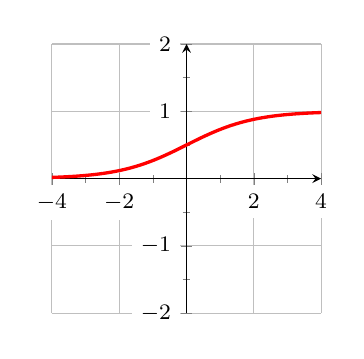
\begin{tikzpicture}
	\begin{axis}[ 
	%title=$\tanh(x)$,
	xmin=-4, xmax=4,ymin=-2, 
	ymax=2, grid=major,
	height=5cm, width=5cm,
	axis line style={latex-latex},
	axis lines=middle,
	ticklabel style={font=\footnotesize,fill=white},
	minor tick num=1,
	scaled ticks=false] 
	\addplot[samples=100,red,very thick] {1/(1+exp(-x))};
	%\addlegendentry{$\tanh(x)$}
	\end{axis}
	\end{tikzpicture}
	
	
	
\subcaption{sigmoid}
\end{subfigure}
\hfill
	\begin{subfigure}[b]{0.24\linewidth}
		
		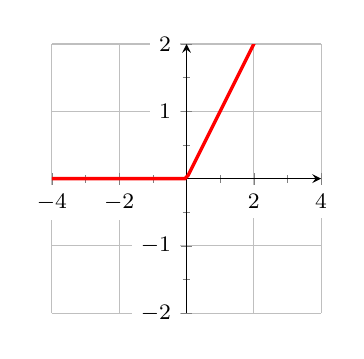
\begin{tikzpicture}
		\begin{axis}[ 
		%title=$\tanh(x)$,
		xmin=-4, xmax=4, ymin=-2, ymax=2, grid=major,
		height=5cm, width=5cm,
		axis line style={latex-latex},
		axis lines=middle,
		ticklabel style={font=\footnotesize,fill=white},
		minor tick num=1,
		scaled ticks=false] 
		\addplot[samples=100,red,very thick] {max(0,x)};
		%\addlegendentry{$\tanh(x)$}
		\end{axis}
		
		\end{tikzpicture}

\subcaption{ReLU}
	\end{subfigure}
\hfill
		\begin{subfigure}[b]{0.24\linewidth}
			
		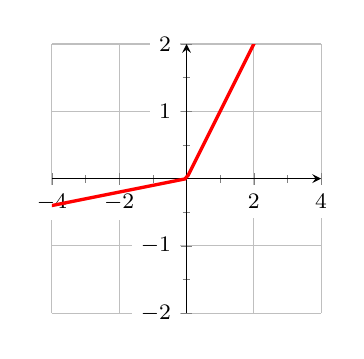
\begin{tikzpicture}
		\begin{axis}[ 
		%title=$\tanh(x)$,
		xmin=-4, xmax=4,ymin=-2, 
		ymax=2, grid=major,
		height=5cm, width=5cm,
		axis line style={latex-latex},
		axis lines=middle,
		ticklabel style={font=\footnotesize,fill=white},
		, xticklabel style={anchor=north},
		minor tick num=1,
		scaled ticks=false] 
		\addplot[samples=100,red,very thick] {max(0,x)+min(0,0.1*x)};
		%\addlegendentry{$\tanh(x)$}
		\end{axis}
		
		\end{tikzpicture}
		\subcaption{Leaky ReLU}
		\end{subfigure}